\chapter{Static Solutions}\label{ch: static solutions}

Within our study of equations of state, we want to see which predictions each unique equation makes about the macroscopic (observable) properties of a neutron star. To do so, we introduce the Tolman-Oppenheimer-Volkoff (TOV) equations, a time independent description of a spherically symmetric neutron star. By solving the TOV equations, we can calculate theoretical observables, such as the total mass and radius of an individual star, and compare them to empirical data gathered from real neutron stars. This chapter will introduce the TOV equations, show how they are solved, and how through analysis we can determine the aforementioned observable quantities of note.

\section{The Tolman-Oppenheimer-Volkoff (TOV) Equations}

The Tolman-Oppenheimer-Volkoff (TOV) equations are the below system of two coupled differential equations
\begin{align}\label{eqn: tov}
    \dv{m}{r} = 4\pi r^2 \epsilon, \quad \dv{P}{r} = -\frac{(4\pi r^3 P + m)(\epsilon + P)}{r^2 (1-2m/r)}.
\end{align}
Within these equations, there are four important variables: the \textit{radial coordinate}, $r$, the \textit{mass}, $m$, the \textit{pressure}, $P$, and the \textit{energy density}, $\epsilon$. Within this model, we consider neutron stars to be spherically symmetric; this means that only the distance from the center of the star is important. Furthermore, the radius $r$ is the independent variable; therefore, the other variables can be written as functions of this radius: $m=m(r)$, $P=P(r)$, and $\epsilon=\epsilon(r)$.

The parameter $m$ is defined as the total amount of energy within a spherical shell of radius $r$. Technically, this is not identical to mass; however, due to Einstein's mass-energy equivalence, it is common and convenient to call this parameter mass. This paper will continue this convention. 

At this point, we have two variables remaining, yet only one unaccounted for equation in this system. It is here we can finally show the importance of the equation of state within our neutron star calculations. Within this system, the energy density and pressure are related directly by an equation $\epsilon = \epsilon(P)$ known as ``the equation of state'' (EOS). This relationship is important because it allows us to determine the current value of $\epsilon$ if we already know the value of pressure.\footnote{ Practically, it is also easy to find pressure if we know energy density, however that is not necessary in this calculation.} The EOS will be derived and analyzed in depth in the later sections of this paper; at this point, however, it is important to understand that the EOS encodes the interactions between the particles within the neutron star, and based on the model used to describe those interactions, it will change. For this derivation, we leave the EOS as a general function. After including an EOS in our TOV equations, we now just have two variables to evolve: $m$ and $P$.

To determine a solution to the system of equations in \eqref{eqn: tov}, we need will solve an initial value problem. As we want to know information about the star from its center radially outward, we therefore need initial conditions for both $m$ and $P$ at the center of the star, $r=0$. Determining an initial condition for $m(r=0)$ is straightforward; as $m$ represents the total mass contained within a radius $r$, at the center of the star, as no mass is enclosed, so $m(0)=0$. We treat the initial condition for $P$, $P(0)$, called the \textit{central pressure}, as a free parameter. Every static solution is uniquely specified by a value of the central pressure; thus, we simply choose a reasonable value (typically $P(0)$ somewhere between $\SI{e-6}{GeV^4}$ and $\SI{e-1}{GeV^4}$) and begin our integration. These initial conditions are summarized as
\begin{align}\label{eqn: tov ic}
    m(0) = 0, \quad P(0) \in [\SI{e-6}{GeV^4}, \SI{e-1}{GeV^4}].
\end{align}

When beginning our integration, we cannot, however, start directly at $r=0$, as $\dv*{P}{r}$ has terms containing $1/r$. To determine $\dv*{P}{r}$ at $r=0$, we would need to take a limit; however, numerically, we can avoid this by starting at very small $r$. Therefore, we simply start at a tiny value of $r$, say $r\approx\SI{e-8}{}$. This effectively approximates the limit and is accurate enough for our purposes.

We want our integration to terminate once we reach the edge of the star, as we are not interested in anything beyond that point. To find this outer edge, we define the total radius of the star, $R$, as the radius when 
\begin{align}
    P(R) = 0.
\end{align}
In practice, once we reach a very small pressure, $P \sim \SI{e-12}{}$, we can end the integration. Once we have found $R$, we can determine $M = m(R)$, the total mass enclosed at radius $R$. The total mass $M$ and total radius $R$ are important to our analyses of different equations of state, as they represent experimentally observable properties of real neutron stars. These theoretically calculated properties can be compared to observed properties to gauge the validity of any given equation of state.

By determining a solution to the TOV equations, we calculate something called a ``static solution,'' a time independent description of a neutron star. A solution contains three curves: $m(r)$, $\epsilon(r)$, and $P(r)$. Of most importance are the pressure and energy density curves; however because they are related by the EOS, we only need to save one curve, as we can simply calculate the other when desired.


\section{Computing Static Solutions}\label{sec: tov, computing static solutions}

To compute static solutions, we use numerical integration techniques for solving ordinary differential equations (ODEs). In this situation, we use a specific technique known as the fourth-order Runge-Kutta algorithm (RK4). First, we need a differential equation of the form
\[\dv{y}{x} = f(x, y),\]
where $x$ is the independent variable, and $y$ is the function whose solution we wish to find. Importantly, $y$ can be a vector valued function, so we can evolve a system of coupled differential equations using this method. Given a current value of the function, $y(x)$, RK4 allows to find an approximate value of the function a small step $h$ forward in $x$: $y(x+h)$. Computationally, the algorithm is
\begin{align}\label{eqn: rk4}
    y(x_i+h) \cong y(x_i) + \frac{1}{6}(k_1 + 2k_2 + 2k_3 + k_4),
\end{align}
where
\begin{align}
    k_1 & = h f(x_i, y_i),\nonumber\\
    k_2 & = h f(x_i+h/2, y_i+k_1/2),\nonumber\\
    k_3 & = h f(x_i+h/2, y_i+k_2/2),\nonumber\\
    k_4 & = h f(x_i +h, y_i + k_3).\nonumber
\end{align}
If $y$ is a vector valued function, then each of the $k_i$ values will also be vector valued. To determine a solution for $y$, we start with an initial condition, $y(x_0)$. Then, after choosing a step size $h$, we use the initial value of $y$ to determine $k_1$ through $k_4$. Finally, we can then calculate $y(x_0+h)$ using \eqref{eqn: rk4}. At this point, we repeat the process using the newly calculated values of $y$ as our initial data, allowing us to calculate the value of $y$ one more step forward. This algorithm is repeated as necessary.

For our system of coupled ODEs in \eqref{eqn: tov}, the independent variable is $r$ and our function is the vector is $y = (m, P)$. Using the initial conditions $y_0 = (0, P_0)$ from \eqref{eqn: tov ic}, we can begin our integration from the center of the star and work outwards with step size $h = \Delta r$, a small step in the radial direction. We continually use the newly calculated values of $y$ at some radius $r$ to determine the value of $y(r+\Delta r)$. As we want the integration to terminate when $P$ gets too small, every time we calculate new values, we check to make sure that $P$ is still in an acceptable range, and if it is too small, we terminate.


This method allows us to generate static solution curves for various equations of state $\epsilon (P)$ and central pressures $P(0)$. For an equation of state called ``SLy'' from \autocite{SLy_2004} with a central pressure $P(0) = \SI{e-4}{GeV^4}$, an example of the resulting curves for pressure and energy density are shown in \autoref{fig: SLy static solutions}.

\begin{figure}[h!]
    \centering
    \begin{subfigure}{.5\textwidth}
        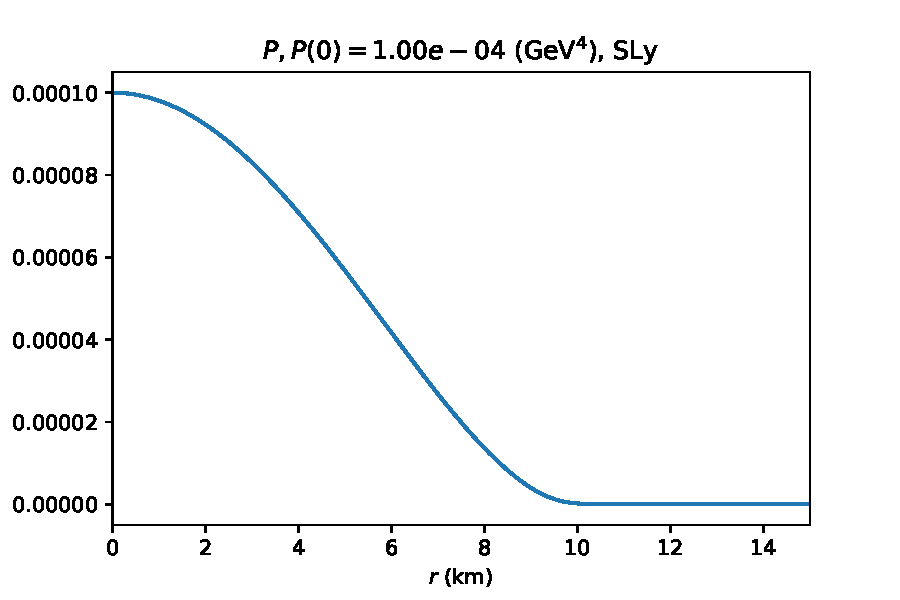
\includegraphics[width=\textwidth]{images/tov/SLy_P,p0_0.0001.pdf}
    \end{subfigure}%
    \begin{subfigure}{.5\textwidth}
        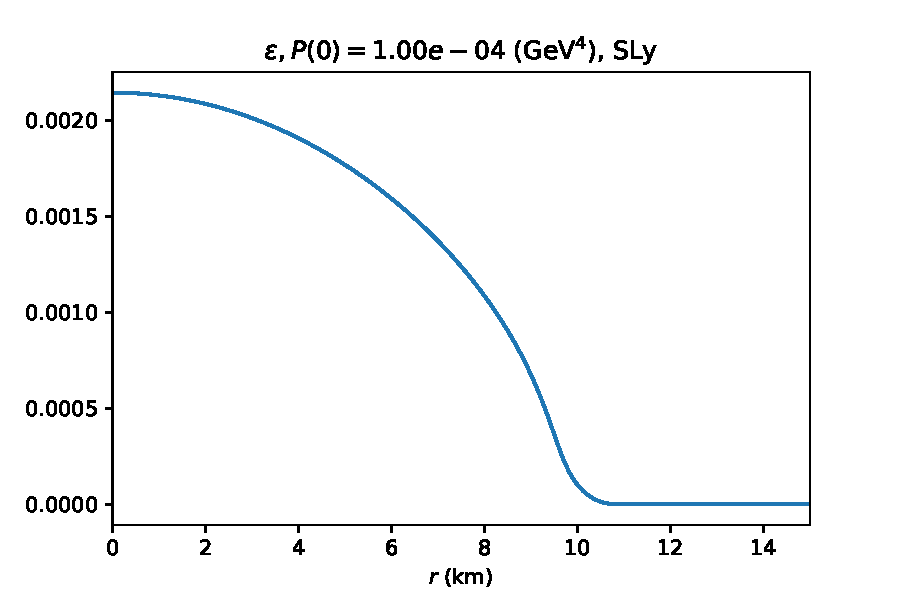
\includegraphics[width=\textwidth]{images/tov/SLy_rho,p0_0.0001.pdf}
    \end{subfigure}
    \caption{The pressure $P$ (left) and energy density $\epsilon$ (right) for $P(0) = \SI{e-4}{GeV^4}$ with equation of state SLy from \autocite{SLy_2004}.}
    \label{fig: SLy static solutions}
\end{figure}

By observation, in \autoref{fig: SLy static solutions}, we can see that the total radius, $R$, is about $\SI{10}{km}$, as this is when the pressure goes to zero. Using this value, we can determine what the total mass is by plugging it into the mass function (not pictured). These values are vital within \autoref{sec: tov,AoSS}.

\section{Analysis of Static Solutions}\label{sec: tov,AoSS}

% Using the results from \autoref{sec: tov, computing static solutions}, we can build up a procedure to produce curves that tell us what kinds of stars an equation of state will predict. 

In \autoref{fig: SLy static solutions}, we looked at one static solution produced using a realistic equation of state called SLy. The decision to use SLy was simply exemplary in this case; we could have used a different equation of state and the static solutions therefore would have been different. To determine the predictions that an individual equation of state will make over a range of values, it is impractical to simply look at static solution curves, such as those in \autoref{fig: SLy static solutions}. Instead, we look at the macroscopic properties, $M$ and $R$, that each predicts over a wide range of central pressure values.

To do this, we create a range of central pressure values, approximately $P(0)\in [\SI{e-6}{}, \SI{e-1}{}]$, s. In practice, it is useful to use a logarithmic range of values, such that the values are more densely packed near $P=\SI{e-6}{}$; within our code, we use the \code{numpy} function \code{logspace} to create an array of values with logarithmic spacing. Now, we can iterate through these pressure values and create static solutions for each central pressure. For every static solution, we integrate until we find $R$, at which time we also calculate $M$. These values are stored, along with the central pressure value from which they were produced.

Using these values, we plot two curves: $M$ vs. $P_0$ and $M$ vs. $R$. These are shown in \autoref{fig: tov, SLy mac curves}.

\begin{figure}[h!]
    \centering
    \begin{subfigure}{.5\textwidth}
        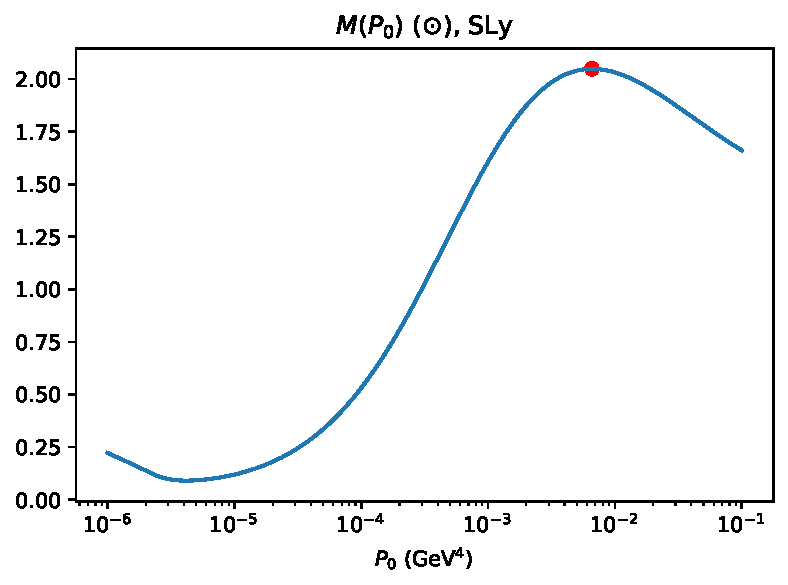
\includegraphics[width=\textwidth]{images/tov/p0_analysis,SLy.pdf}
    \end{subfigure}%
    \begin{subfigure}{.5\textwidth}
        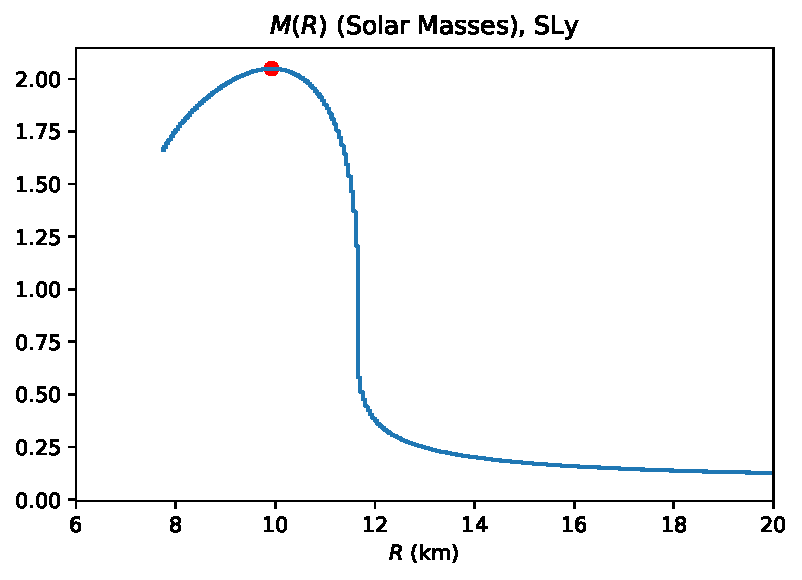
\includegraphics[width=\textwidth]{images/tov/r_analysis,SLy.pdf}
    \end{subfigure}
    \caption{The curves $M$ vs. $P_0$ (left) and $M$ vs. $R$ (right) for the SLy equation of state from \autocite{SLy_2004}.}
    \label{fig: tov, SLy mac curves}
\end{figure}

From these curves, we deduce three special values: the \textit{critical pressure}, the \textit{critical radius}, and the \textit{critical mass}. The critical mass is the maximum mass that the EOS predicts, and the critical pressure and critical radius are the pressure and radius, respectively, where the critical mass is reached. The critical mass and critical radius are used as measuring sticks for how realistic an equation of state is; if they are on the same order as the largest neutron stars that have been actually observed, the equation of state is considered to be a candidate for a ``correct'' description of the star. Usually, the critical mass is on the order of about 2 solar masses, while the critical radius is on the order of about \SI{10}{km}. Within the above plots, we have converted the units of radius to \SI{}{km} and the units of mass to \textit{solar masses}, denoted $\odot$, where $\SI{1}{\odot} = \SI{1.989e+30}{kg}.$

In \autocite{SLy_2004}, besides the SLy EOS, there is an additional EOS called FPS, derived and implemented in a similar fashion, just with a different parameterization. Furthermore, in another paper by the same authors, \autocite{BSk_2013}, there are three additional EOSs of similar form. All of these EOSs are considered realistic equations of state and are computed by creating analytical fits from empirical observational data from neutron stars. From previous work, we have these EOSs implemented, so for demonstration, we have overlaid the mass-radius and mass-pressure curves to demonstrate the differences in predictions of different equations of state. These curves are shown in \autoref{fig: tov, all eos analyses}.

\begin{figure}[h!]
    \centering
    \begin{subfigure}{.5\textwidth}
        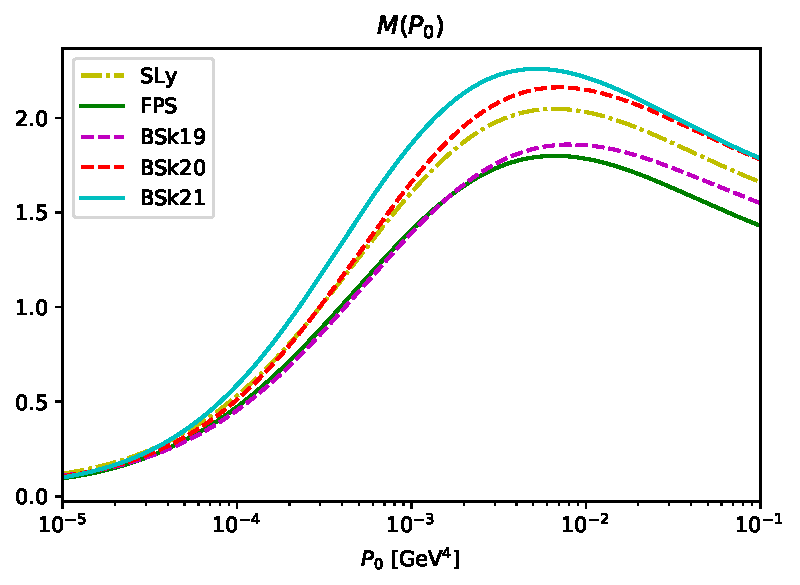
\includegraphics[width=\textwidth]{images/tov/p0_analysis,all.pdf}
    \end{subfigure}%
    \begin{subfigure}{.5\textwidth}
        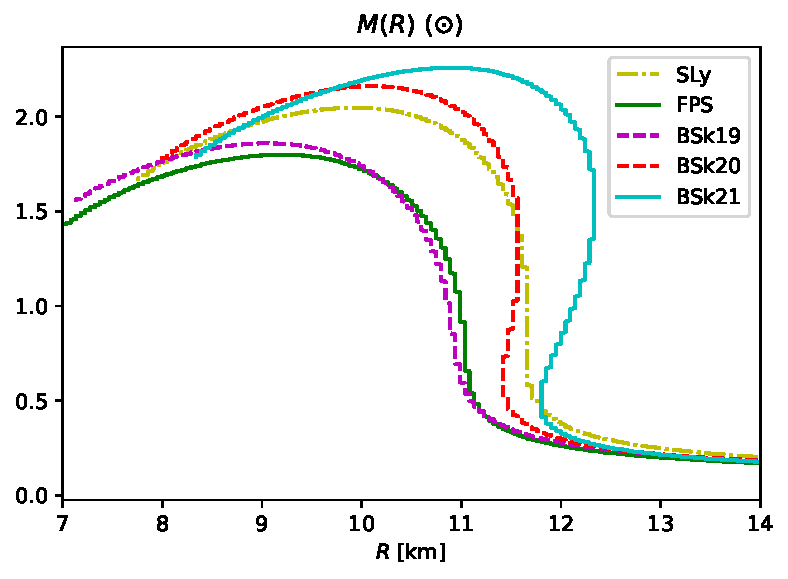
\includegraphics[width=\textwidth]{images/tov/r_analysis,all.pdf}
    \end{subfigure}
    \caption{The mass-central pressure (left) and mass-radius (right) diagrams for the five equations of state from \autocite{SLy_2004,BSk_2013}. Mass given in solar masses ($\odot$).}
    \label{fig: tov, all eos analyses}
\end{figure}

As we can see from looking at these curves, these EOSs produce curves that are qualitatively similar yet with slightly different numerical values. For example, the EOS BSk21 predicts a maximum mass of $\SI{2.26}{\odot}$ and a critical radius of $\SI{10.8}{km}$, while FPS predicts a maximum mass of $\SI{1.80}{\odot}$ with a critical radius of \SI{9.2}{km}, with the predictions of the three other EOSs falling somewhere in between. We see that these five models therefore produce results that are well within the same order of magnitude with similar qualitative features, however their predictions are most definitely the same. As the actual EOS within a neutron star is unknown, these differences are non-trivial and studying them may lead to a better understanding of the real interactions within neutron stars in the future.

\section{Implementation of Static Solutions and Analyses}

During this section, the code given in \autoref{ch: tov code} will be referenced extensively. Any line numbers, unless specified, refer to this code

To begin, we wanted to create a program that would allow for an arbitrary equation of state and central pressure to chosen and would then produce the corresponding static solution. In line 42, the boolean flag \code{make\_static\_solution} selects this mode, and the central pressure specified in line 48 is the central pressure used as an initial condition in the TOV equations. Furthermore, lines 12 through 39 are used to specify which equation of state is to be used.

The EOSs that we use when solving the TOV equations are not actually analytical equations or functions defined within our code. Instead, we have various \code{.txt} files that contain tabulated values of both $\epsilon$ and $P$. When a given EOS is chosen, we read in that text file and use the SciPy function \code{interp1d} to create an ``interpolation function.'' This function takes the $P$ values as independent variables and $\epsilon$ values; then, whenever this function is called throughout the remainder of the code, it will use an interpolation routine to predict an approximate value of $\epsilon$ for an inputted value of $P$. The implementation of this procedure is between lines 70 and 90.\footnote{There are two special EOSs called the ``ultra-relativisitic equation of state'' (UR EOS) and ``polytropic equation of state'' that are purely analytical. As this is the case, in lines 84-90, we choose the analytical equations of state if either the UR or polytropic EOS is chosen, and otherwise we use the interpolating function as described above.}

We also initialize other important parameters. We want to produce static solutions from a minimum $r$ value ($r=0$)\footnote{As mentioned before, we must choose an actual $r_0$ value that is just slightly bigger than 0, as using $r=0$ in \eqref{eqn: tov} would cause the denominator of $\dv*{P}{r}$ to be undefined.} out to a maximum specified value, in this case, $r=200$. Furthermore, we want our points spaced at a regular interval, small enough to give us adequate precision, but not too small as to hinder the code's speed too much. Therefore, we choose our radial step size, \code{dr}, to be $0.02$. Then, we create an array of these $r$ values, spaced out at the desired step size. Finally, we set the initial condition of $m$ to 0. This is all given between lines 56 and 64

After the necessary parameters are initialized, we define the functions necessary for integration. First, on line 101, we define the vector funciton \code{f\_onefluid}, a function of both the independent variable $r$ and vector function $y$. Then, $y$ is unpacked into $m$ and $P$, the equation of state is used to determine $\epsilon$ (or, in the code, called \code{rho}), and finally the right-hand sides of the equations in \eqref{eqn: tov} are evaluated and returned as a tuple. Secondly, we define a function called event, which is also a function of $r$ and $y$. This function compares the current $P$ value to a parameter called \code{p\_tol}; \code{p\_tol} is the smallest effective pressure value for which we consider the pressure to have gone to zero. On line 61, we define this threshold to be \SI{e-11}{}. This function will be used to terminate the integration once we have reached the edge of the star.

Now, on line 115, we begin the integration for our static solution. We open files, with the current parameters we are using (such as the radial step size and central pressure) in the file name. On line 128, we use a SciPy function called \code{solve\_ivp} ro perform the numerical integration (using the Runge-Kutta method) and return an array containing the solutions for both $P$ and $m$. We use \code{solve\_ivp} and do not implement RK4 on our own for speed purposes; \code{solve\_ivp} has special optimizations in regards to step size under the hood that make the calculations more efficient when the values are very large and very small. Importantly, we pass the \code{event} function to \code{solve\_ivp} as a parameter; throughout the integration, \code{solve\_ivp} checks to see if the pressure has dropped below the tolerance, and if it has, it terminates the integration there. Then, we write the static solution to a file, where we fill out any points after the termination but before the $r_\text{max}$ value with zeros. These files are then subsequently read into a different program for plotting, producing the curves like those shown in \autoref{fig: SLy static solutions}.

For the analyses (i.e. producing the mass-radius and mass-pressure curves), we use a similar procedure to that described above, instead we iterate over a wide range of pressure values. If the boolean flag \code{p0\_analysis} is set on line 43, then we will enter the loop on line 149. From there, we loop over all $P_0$ values in the \code{p0\_vals} array, creating a static solution for each and saving the critical mass, critical radius, and critical pressure values to a file. Then after the completion of the loop, we can use an additional program to create a plot. When calculating the critical mass, we use an optimization routine to determine the top of the mass-pressure or mass-radius curve more precisely, and use that calculated critical value to determine the critical radius or pressure, respectively. 

For the remainder of this project, this program will be used to produce the plots and analyses for the equations of state that we derive.

